\chapter{Graphene.js: Building Reusuable Web Components for Data Visualization}

\section{Purpose}

The purpose of this chapter is to introduce Graphene.js \autocite{gu2014graphene}, a framework for creating data-driven visualizations and user interfaces.
In addition, the Graphene.js approach to data visualization is contrasted to currently established JavaScript drawing libraries.
Graphene is the key component of the user interface for all other applications described in this body of work.

Graphene is open source and available on GitHub.

\section{Motivation}

Graphical representations of information are valuable for presenting complex information quickly and clearly. \autocite{newsom2007public, smiciklas2012power}
They can vastly improve comprehension by using graphics to enhance the human visual system’s ability to see patterns and trends. \autocite{heer2010tour, sears2007human}
Meanwhile, the Internet and World Wide Web \autocite{berners2000weaving} has become perhaps the most powerful medium for information sharing. \autocite{bollacker1998citeseer, wilkinson2003motivations, page1999pagerank}
Modern web applications have many advantages over traditional desktop applications.
Software developers typically face a challenge in deploying software applications to their clients (Figure~\ref{fig:deployment-problem}).
End users may use a wide variety of platforms, such as Apple OS X, Microsoft Windows, and Linux for desktop computers and Apple iOS, Google Android, and Microsoft Windows Phone for mobile devices.
Each platform has a different pattern for building native binaries, which requires special expertise and is an obstacle particularly for smaller development teams and research labs.
Web applications are inherently cross platform, available on all devices with a capable web browser (Figure~\ref{web-app-deployment}).
Updates are also delivered immediately, which is typically not the case for desktop softwares.
Thus, HTML5 web applications are a compelling platform for biomodeling applications as well.

\begin{figure}
  \centering
  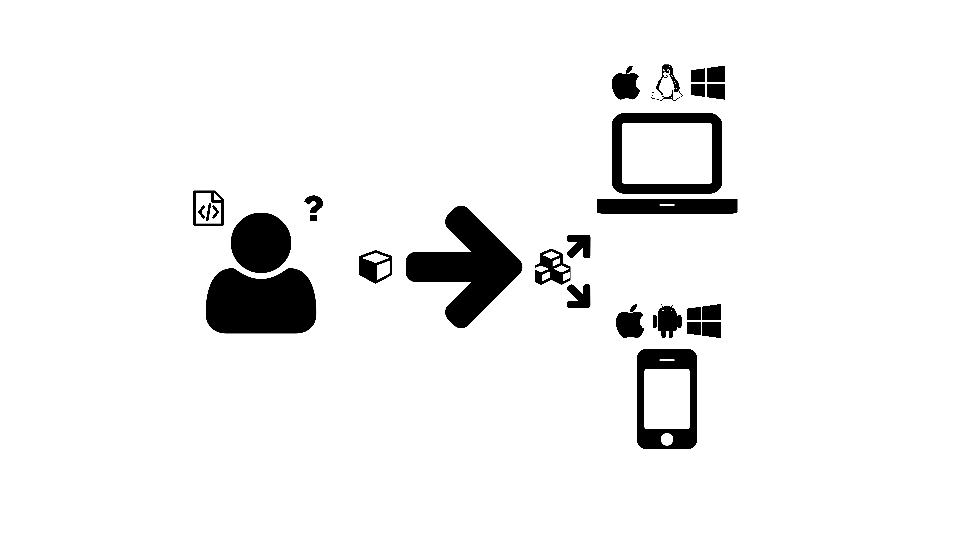
\includegraphics[width=\textwidth,natwidth=610,natheight=642]{images/deployment-problem.png}
  \caption{Software developers often face a challenge in deploying their code base to end users due to the widespread use of multiple platforms.}
  \label{fig:deployment-problem}
\end{figure}
\begin{figure}
  \centering
  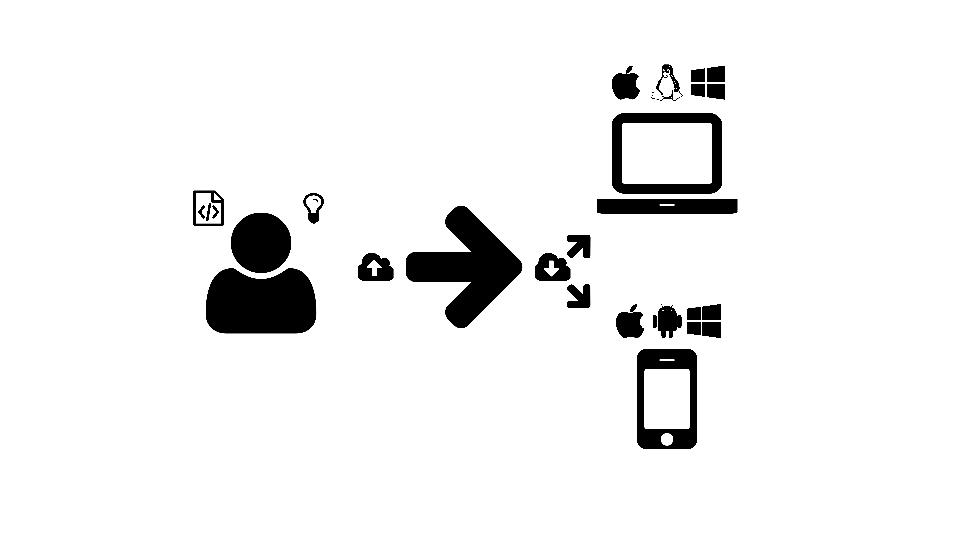
\includegraphics[width=\textwidth,natwidth=610,natheight=642]{images/web-app-deployment.png}
  \caption{Web applications solve the cross-platform problem.}
  \label{fig:web-app-deployment}
\end{figure}

\subsection{Few systems biology software packages are built using HTML5 web technologies}
Modeling standards and open source software packages, as reviewed in  Software in chapter~\ref{chap:background}, have been a boon to the biomedical research community.
While there are a wide variety of powerful tools that have been developed over the years, there is a distinct lack of web applications.
One way to get a sense of the current landscape of modeling software is to consider the SBML Software Guide \autocite{sbml2014software}, which has conveniently organized and characterized publicized SBML compatible software.
Of the 96 closed-source software packages listed in the Software Guide, only 24 contain any type of web based features and only one can be considered an HTML5 web application \autocite{olivier2004web}.
Of the 166 free and open source softwares listed, just 37 contain any web capabilities, and none of which are an HTML5 application.
\subsection{Systems biology software is complex and building complex web applications is difficult}
There are several obstacles to building biomodeling web applications, which may explain the absence of web applications in the biomodeling domain.
Scientific libraries that most biomodeling software depends on have been intended for desktop use, which can also be used server-side in a web application, but requires additional expertise.
Furthermore, designing and implementing complex graphical user interfaces (GUIs) on the web is a nontrivial engineering challenge.
As discussed in section~\ref{sec:html5} HTML was originally designed as a markup language for communicating static pages that contain text and limited amounts of media, while using CSS for styling.
The rise of JavaScript support within browsers allowed web pages to evolve more interactive behaviors, leading eventually to the web applications of today.
However, JavaScript was originally intended for simple scripts which manipulate the DOM, and this legacy has lead to challenges in scaling increasingly complex JavaScript applications.

\subsubsection{JavaScript code bases that treat the DOM as data model are difficult to scale}

\begin{figure}
  \centering
  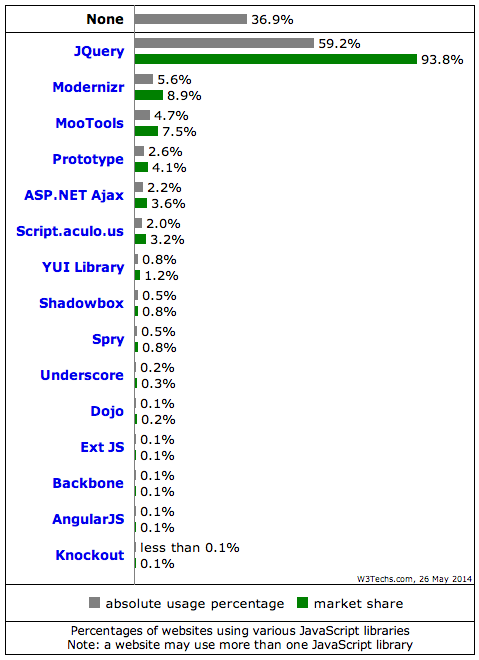
\includegraphics[width=\textwidth,natwidth=610,natheight=642]{images/jquery-marketshare.png}
  \caption{Market share client-side JavaScript libraries as of May 2014. \autocite{w3techs2014javascript}}
  \label{fig:jquery-marketshare}
\end{figure}

By far, the most popular client-side JavaScript library is jQuery. \autocite{w3techs2014javascript}
Of the 59.2\% of websites that contain JavaScript, JQuery is present in 93.8\% of them (Figure~\ref{fig:jquery-marketshare}).
In web applications that primarily rely on JQuery, the most common design pattern is to treat the DOM as the data model (DOMAM).
In DOMAM, controller logic acts on the DOM directly, creating, updating, and deleting DOM components when the application data model changes.
DOMAM style applications are easy to implement for small applications, but as they grow larger and more complex, the lack of separating the model and view leads to difficulties for software maintenance and continued development.
Section~\ref{sec:declarative-vs-imperative} provides more description and examples on the weaknesses of the DOMAM pattern, as it is perhaps easier to understand when compared to the alternative solution.

\subsection{Most existing drawing libraries follow the jQuery DOM manipulation pattern and are less suited for complex and customizable visualizations}
A key component of GUI for computational systems biology application is in its bio-network graph layout.
In order to reduce duplication of code effort and promote programming best practices, it is desirable to use a software library when solving recurring software problems.
However, most JavaScript drawing libraries encourage the DOMAM pattern or lack customization options.
Being able to customize the visual layout allows for greater design control of an application's UI. 
Better web designs are important because it may increase user engagement and likelihood of revisiting. \autocite{rosen2004website}


\section{Solution}

\subsection{Graphene.js allows for easily customizable and reusuable web diagrams}
Graphene.js addresses these issues by using a different approach.
Graphene creates interactive diagrams through two-way-binding of the application data model to a customizable SVG template.
Thus, no custom rendering engine is required as it is performed by the browser, and the rich SVG vocabulary (which may be created through a text editor or through a graphical SVG drawing program) may be used to define nearly any type of edge, arrow marker, or Bezier curve.
Graphene templates may also be customized for visualizations beyond node-edge graphs, such as charts and animations.


Cytoscape.js \autocite{cytoscape2014js} is a graph drawing library and a potential choice for network visualization. 
It contains an impressive HTML5 Canvas based rendering engine, but currently lacks the ability to customize the following:

\begin{itemize}
\item Color gradients for nodes
\item Marker ends and node shapes beyond a predefined set
\item Control points for Bezier curves
\item Placement of edge start and end points
\end{itemize}

In addition, since Cytoscape.js produces a canvas drawing and not DOM elements, the graph elements are unable to be used with other JavaScript libraries (for example a popover plugin that acts on each node) nor bound to custom events.
Cytoscape Web \autocite{cytoscape2014web} is a similar library, but is based on Adobe Flash, which limits its utility for cross platform deployment.

\subsection{Declarative vs. Imperative: Data-binding over DOM manipulation}
\label{sec:declarative-vs-imperative}

Graphene uses Angular.js \autocite{google2014angular} to provide a Model-View-Controller \autocite{krasner1988description} interface for implementing layouts.
Here we will discuss the differences between the DOMAM/jQuery pattern and Angular MVC approach, which will help explain the design decisions behind Graphene.
Consider this jQuery example of fetching JSON data from an endpoing:

\begin{lstlisting}[language=JavaScript]
$.ajax({
  url: '/myData.json',
  success: function(data, status) {
    $('ul#log').append('<li>Data Received!</li>');
  }
});
\end{lstlisting}

\texttt{\$.ajax} performs an asynchronous HTTP (Ajax) request, which accepts the location of the data endpoint as \texttt{url} and the callback function as \texttt{success}.
Upon receiving data, we simply append a new \texttt{<li>} into the portion of the DOM that matches the \texttt{'ul\#log'} CSS selector string.
Thus, the view may look something like this:

\begin{lstlisting}[language=html]
<ul class="messages" id="log">
</ul>
\end{lstlisting}

Alternatively, the Angular approach to accomplishing this same task would look something like this:

\begin{lstlisting}[language=JavaScript]
$http( '/myData.json' ).then( function ( response ) {
  $scope.log.push( { msg: 'Data Received!' } );
});
\end{lstlisting}

With the corresponding view of:

\begin{lstlisting}[language=html]
<ul class="messages">
  <li ng-repeat="entry in log">{{ entry.msg }}</li>
</ul>
\end{lstlisting}

The major difference in the Angular approach is that the callback function does not manipulate the DOM directly.
The controller is only responsible for updating the data model, \texttt{\$scope.log}.
Thus, the view, with the help of the \texttt{ng-repeat} directive, is reponsible for responding for updating itself to reflect changes in the model.
The controller logic has nothing to do with how the data is actually displayed, and the view will respond to the data regardless of where or how it was changed.
By following Separation of Concerns, a design principle for creating modular programs, the result is simplified development and maintenance.
For example, the view can be swapped out for the following without any need to change the controller logic.

\begin{lstlisting}[language=html]
<div class="messages">
  <div class="alert" ng-repeat="entry in log">
    {{ entry.msg }}
  </div>
</div>
\end{lstlisting}

Similarly, Graphene brings the Separation of Concerns pattern to drawing on the web.
Consider how one must use the drawing API of a well established drawing library, Raphael.js. \autocite{sencha2014raphael} in creating a simple node-edge diagram (Figure~\ref{fig:graphene-simple}).

\begin{figure}
  \centering
  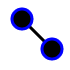
\includegraphics[width=70px,natwidth=610,natheight=642]{images/graphene-simple-70x70.png}
  \caption{A simple node-edge graph diagram.}
  \label{fig:graphene-simple}
\end{figure}

\begin{lstlisting}[language=JavaScript]
// Creates a canvas on the element with id of 'canvas'
var paper = Raphael('#canvas', 100, 100);

// Creates circle node at x = 20, y = 20, with radius 10
var n1 = paper.circle(20, 20, 10);
// Sets the fill attribute of the circle to black
n1.attr("fill", "black");
// Sets the stroke attribute of the circle to blue
n1.attr("stroke", "blue");

// Creates circle node at x = 50, y = 50, with radius 10
var n2 = paper.circle(50, 50, 10);
// Sets the fill attribute of the circle to black
n2.attr("fill", "black");
// Sets the stroke attribute of the circle to blue
n2.attr("stroke", "blue");

// Creates a line from n1 to n2
var edge = paper.path("M20 20L50 50")
edge.attr("fill", "black");
edge.attr("stroke", "black");
\end{lstlisting}

In contrast, the below is the Graphene approach for drawing the same diagram. \autocite{gu2014grapheneSimple}

\begin{lstlisting}[language=JavaScript]
// Data Controller
// Array of node objects
$scope.nodes = [{
  id: 'n1',
  x: 20,
  y: 20
}, {
  id: 'n2',
  x: 50,
  y: 50
}];

// Array of edges, each containing references to source and target nodes
$scope.edges = [{
  source: $scope.nodes[0],
  target: $scope.nodes[1]
}];

// Specify which variables to export to the template
$scope.exports = {
  nodes: $scope.nodes,
  edges: $scope.edges
};
\end{lstlisting}

\begin{lstlisting}[language=html]
<!-- Template -->
<svg width="100" height="100">
  <!-- ng-repeat takes an expression to loop through-->
  <g
    ng-repeat="e in imports.edges"
  >
    <!-- ng-attr-foo takes binds object properties to the DOM element -->
    <line 
      stroke="black"
      stroke-width="3px"
      ng-attr-x1="{{e.source.x}}"
      ng-attr-y1="{{e.source.y}}"
      ng-attr-x2="{{e.target.x}}"
      ng-attr-y2="{{e.target.y}}"
      ></line>
  </g>
  <g 
    ng-repeat="n in imports.nodes"
    ng-attr-transform="translate({{n.x}}, {{n.y}})"
    >
    <circle
      r="10"
      fill="black"
      stroke="blue"
      stroke-width="3px"
    ></circle>
  </g>
</svg>
\end{lstlisting}

The template and controller logic is invoked through the use the \texttt{sg-graphene} directive.

\begin{lstlisting}[language=html]
<sg-graphene template="views/template.html" imports="exports"><sg-graphene>
\end{lstlisting}

Graphene separates the data controller from the view.
Arguably, this format results in code that is more readable, HTML/SVG is used to declaratively define the view.
But perhaps more importantly, separation of concerns is achieved and the view is decoupled from data logic.
Another benefit in the Graphene example is two-way data binding allows the view to be updated when the data changes.
This is a non-trivial task to implement for the Raphael example.

\section{Implementation}

\subsection{Angular.js is used for data-binding and directives}
Graphene contains one main dependency, Angular.js, which is the underlying engine responsible for data-binding and directive definitions.
Data-binding in Angular is done through a process known as "dirty-checking".
Dirty-checking is performed by a series of watchers, which compares new values to its previous value. \autocite{google2014angularScope}
If a value change is detected, the defined change callback function is fired.

At a high level, directives are markers on a DOM element (such as an attribute, element name, comment or CSS class) that tell Angular's HTML compiler to attach a specified behavior to that DOM element or even transform the DOM element and its children. \autocite{google2014angularDirectives, google2014angulardirectives2}
Angular comes a set of directives, such as \texttt{ng-repeat}, but custom ones can also be defined.
A major component of Graphene, \texttt{sg-graphene}, is a custom directive responsible for binding the layout template to objects defined in the controller.
In addition, Graphene also includes helper functions for determining line intersections points for edge placement, and additional directives for imbuing zooming and click-to-drag behavior.



\begin{figure}
  \centering
  \begin{subfigure}[t]{0.45\textwidth}
    \includegraphics[width=\textwidth,page=4,trim=0.37cm 3.65cm 15cm 5cm, clip=true]{images/Figures.pdf}
    \caption{}
    \label{Figure:graphene-logo}
  \end{subfigure}
  \begin{subfigure}[t]{.45\textwidth}
    \includegraphics[width=\textwidth,page=4,trim=10cm 0cm 0cm 1cm, clip=true]{images/Figures.pdf}
    \caption{}
    \label{Figure:graphene-data-binding}
  \end{subfigure}
  \begin{subfigure}[b]{\textwidth}
    \includegraphics[width=\textwidth,page=21,trim=0cm 10cm 4cm 0cm, clip=true]{images/Figures.pdf}
    \caption{}
    \label{Figure:graphene-diagram}
  \end{subfigure}
  \caption{}
  \label{Figure:graphene}
\end{figure}

\subsection{External JavaScript libraries can add functionality}
Graphene can easily be used augmented with external JavaScript libraries.
One example is the use of D3.js \autocite{bostock2014d3} for its force-directed layout algorithm.
D3 uses the Barnes-Hut algorithm for simulating the force system. \autocite{bostock2011d3}

\begin{lstlisting}[language=JavaScript]
// Initalize force coordinate system
var force = d3.layout.force()
  .size([$scope.width || 800, $scope.height || 800]);

// Bind links and nodes to the new force system
force
  .nodes($scope.nodes)
  .links($scope.links)
  .on('tick', function() {
    // Bind callback function that runs on every 'tick' of force layout
    if ($scope.height && $scope.width) {
      // this ensures that no nodes ever leave the outermost edges
      // of the force coordinate system
      _.each($scope.nodes, function(n) {
        n.x = Math.max(n.width, Math.min($scope.width -
          n.width, n.x));
        n.y = Math.max(n.height, Math.min($scope.height -
          n.height, n.y));
      });
    }
    // Triggers a digest cycle so view can update with new node positions
    $scope.$digest();
  })
  // Begin force simulation
  .start();
\end{lstlisting}

\subsection{Yeoman build chain allows for easy development and integration workflows}

Graphene was developed with the Yeoman in order to follow best practices in web development, allow users to easily integrate Graphene within their own codebases, and promote modular design.
Yeoman consist of the web development build tools: yo \autocite{yeoman2014yo}, grunt \autocite{alman2014grunt}, and bower \autocite{twitter2014bower}.
yo consists of a number of community maintained and developed generators that scaffold out new applications, generate Grunt configurations and pulling in relevant Bower dependencies.
Grunt is a task runner, used to build, preview, test, and deploy projects.
Bower is a dependency management system, so developers no longer have to manually download and manage JavaScript packages.

Many tutorial exist online in using these tools.
New users can install Graphene with the simple command \texttt{bower install graphene}.
For the developers and maintainers of Graphene, new versions can be tested and deployed to GitHub through the command \texttt{grunt dist}.

\section{Future Directions}
The trend of where web standards and development is going was one of the major underlying motivators for the Graphene approach.
Directives and data-binding that is provided Angular.js are actually stepping stones for Native HTML Web Components \autocite{w3c2014components}, HTML Templates \autocite{w3c2014templating}, and ECMAScript 6 \texttt{Object.observe} data-binding \autocite{polymer2014templating}.
Thus, the goal of Graphene is to introduce the biomodeling community towards the horizon of modern, functional web applications.

